\documentclass[tikz]{standalone}

\begin{document}
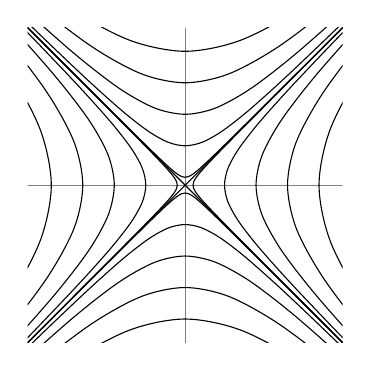
\begin{tikzpicture}
  \clip (-2, -2) rectangle (2, 2);
  \draw[gray] (0, -2) -- (0, 2);
  \draw[gray] (-2, 0) -- (2, 0);
  \foreach \r in {0.1, 0.5, ..., 1.7} {
    \draw[domain=-5:5, smooth] plot ({\r * sinh(\x)}, {\r * cosh(\x)});
    \draw[domain=-5:5, smooth] plot ({-\r * sinh(\x)}, {-\r * cosh(\x)});
    \draw[domain=-5:5, smooth] plot ({\r * cosh(\x)}, {\r * sinh(\x)});
    \draw[domain=-5:5, smooth] plot ({-\r * cosh(\x)}, {-\r * sinh(\x)});
  }
  \draw (-2, -2) -- (2, 2);
  \draw (2, -2) -- (-2, 2);
\end{tikzpicture}
\end{document}
